% state-valent
\documentclass{standalone}

\usepackage{tikz}
\usepackage{tikz-qtree}

\usetikzlibrary{positioning, shapes, arrows.meta, backgrounds, fit}

\begin{document}
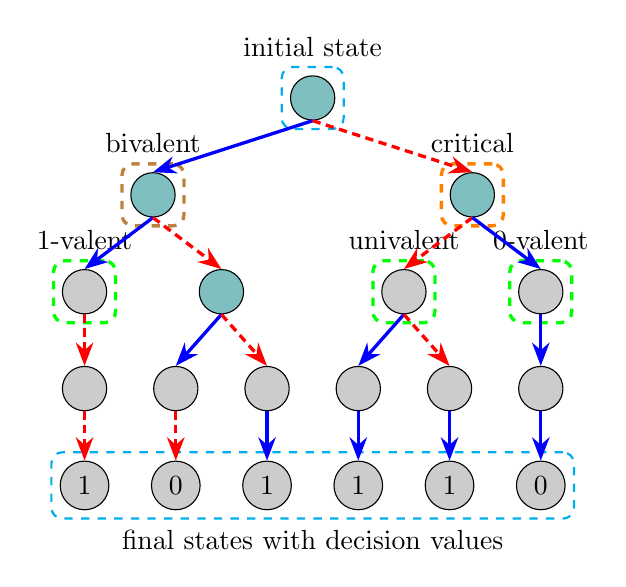
\begin{tikzpicture}[
  univalent/.style = {fill = gray!40},
  bivalent/.style = {fill = teal!50},
  state/.style = {draw, dashed, thick, rectangle, rounded corners, cyan, inner sep = 3pt},
  valent/.style = {draw, dashed, very thick, rectangle, rounded corners, green, inner sep = 3pt},
  every tree node/.style = {draw, circle, minimum size = 16pt, univalent},
  level distance = 35pt, sibling distance = 15pt,
  edge from parent/.style = {blue, draw, very thick, >=Stealth, ->}, 
  bmove/.style = {red, densely dashed},
]
  \Tree [.\node (r) [bivalent] {};
	    [.\node (rl) [bivalent] {};
		[.\node (rll) [] {};
		    \edge[bmove] node[auto = right] {}; 
		    [.\node (rlll) [] {};
			\edge[bmove] node[auto = right] {}; 
			[.\node (rllll) [] {$1$};]
		    ]
	        ]
		\edge[bmove] node[auto = right] {}; 
		[.\node (rlr) [bivalent] {};
		    [.\node (rlrl) [] {};
		      \edge[bmove] node[auto = right] {}; 
		      [.\node (rlrll) [] {$0$};]
		    ]
		    \edge[bmove] node[auto = right] {}; 
		    [.\node (rlrr) [] {};
			[.\node (rlrrl) [] {$1$};]
		    ]
	        ]
	    ]
	    \edge[bmove] node[auto = right] {}; 
	    [.\node (rr) [bivalent] {};
		\edge[bmove] node[auto = right] {}; 
		[.\node (rrl) [] {};
		    [.\node (rrll) [] {};
			[.\node (rrlll) [] {$1$};]
		    ]
		    \edge[bmove] node[auto = right] {}; 
		    [.\node (rrlr) [] {};
			[.\node (rrlrl) [] {$1$};]
		    ]
	        ]
		[.\node (rrr) [] {};
		    [.\node (rrrr) [] {};
			[.\node (rrrrl) [] {$0$};]
		    ]
	        ]
	    ]
  ]

  % init state
  \begin{pgfonlayer}{background}
    \node [state,
      fit = (r),
      label = {[above] {initial state}}] {};
  \end{pgfonlayer}

  % final state
  \begin{pgfonlayer}{background}
    \node [state,
      fit = (rllll) (rlrll) (rlrrl) (rrlll) (rrlrl) (rrrrl),
      label = {[below = 25pt] {final states with decision values}}] {};
  \end{pgfonlayer}

  % univalent
  \begin{pgfonlayer}{background}
    \node [valent,
      fit = (rrl),
      label = {[above] {univalent}}] {};
  \end{pgfonlayer}

  % 1-valent
  \begin{pgfonlayer}{background}
    \node [valent,
      fit = (rll),
      label = {[above] {$1$-valent}}] {};
  \end{pgfonlayer}

  % 0-valent
  \begin{pgfonlayer}{background}
    \node [valent,
      fit = (rrr),
      label = {[above] {$0$-valent}}] {};
  \end{pgfonlayer}

  % bivalent
  \begin{pgfonlayer}{background}
    \node [valent, brown,
      fit = (rl),
      label = {[above] {bivalent}}] {};
  \end{pgfonlayer}

  % critical state
  \begin{pgfonlayer}{background}
    \node [valent, orange,
      fit = (rr),
      label = {[above] {critical}}] {};
  \end{pgfonlayer}
\end{tikzpicture}
\end{document}